\section{Analyse und Aufbereitung der Daten}
Die vorliegende Datei \texttt{thyroid.dat} enthält die Datensätze von 7200
Patienten und soll als Basis für das Training und den Test des zu erstellenden
neuronalen Netzes dienen. Ein Datensatz enthält dabei jeweils 21 verschiedene
Attribute, 15 davon in binärer Form und 6 reellwertig. Folgender Auszug aus der
Datei zeigt den Aufbau der Datensätze: 

\lstinputlisting[firstline=1, lastline=5, caption={Auszug aus der Datei
\texttt{thyroid.dat}}, label={lst:thyroid-auszug}, basicstyle=\footnotesize]{../thyroid.dat}

Es ist hier nicht bekannt, welche Attribute welchen Messwerten entsprechen - 
dieses Wissen wird für die Lösung der Aufgabe auch nicht benötigt. Wie bereits 
eingangs erwähnt, stellt die hohe Anzahl von Attributen eine erste 
Schwierigkeit dar. Weiterhin bereiten die extrem ungleich verteilten Klassen 
Probleme für herkömmliche statistische Methoden. Die letzte Spalte eines Datensatz
enthält dabei die zum Datensatz gehörige Klasse, derer es insgesamt drei gibt:

\begin{itemize}
  \item 1: "`hypothyroid"' (Schilddrüsenunterfunktion),
  \item 2: "`hyperthyroid"' (Schilddrüsenüberfunktion),
  \item 3: "`normal"' (normale Schilddrüsenfunktion).
\end{itemize}

Um zunächst einen groben Überblick über die Daten zu erhalten, wird zunächst die
Verteilung der Datensätze auf die einzelnen Klassen untersucht. Die Situation
stellt sich wie in Tabelle \ref{tbl:klassen-verteilung} aufgezeigt dar.

\begin{table}
	\sffamily
	\centering
	\footnotesize
	\begin{tabular}{lll}
		\toprule
		\multicolumn{1}{@{}N}{Klasse Nr.} &
		\multicolumn{1}{@{}N}{Anzahl} &
		\multicolumn{1}{@{}N}{Anteil [\%]} \\
		\midrule\addlinespace
		
		1 & 166 & 2,3\\
		2 & 368 & 5,1\\
		3 & 6666 & 92,6\\
		
		\addlinespace\bottomrule
		\end{tabular}

  \label{tbl:klassen-verteilung}
\caption{Verteilung der Datensätze auf die drei Klassen} 
\end{table}

\subsection{Aufteilung der Daten in Trainings- und Testdaten}
Üblicherweise werden die verfügbaren Daten zufällig aufgeteilt in eine 
Trainings- und eine Testdatenmenge. Mithilfe der Trainingsmenge wird das 
neuronale Netz erstellt und trainiert. Die Testdatenmenge dient dazu, die 
Qualität des Netzes (in Bezug auf die Vorhersagefähigkeiten) abschließend zu 
überprüfen. Es muss doch gerade in dieser Aufgabe darauf geachtet werden, dass 
die Aufteilung der Daten korrekt erfolgt. Denn betrachtet man die Verteilung 
der Datensätze auf die einzelnen Klassen, so erkennt man, dass in der Klasse 3 
die weitaus meisten Datensätze vorhanden sind (s. auch Abbildung 
\ref{fig:klassen-verteilung}). Würde man nun die Daten blindlings zufällig 
aufteilen, so erhielte man mit großer Wahrscheinlichkeit verfälschte 
Ergebnisse, da ja die meisten Datensätze in der Klasse 3 lägen. Daher wird hier 
so vorgegangen, dass die Daten zunächst in die Klassen aufgeteilt werden und 
anschließend aus jeder dieser drei Untermengen ein gleicher Prozentsatz an Datensätzen 
in den Trainigsdatenpool übernommen wird. Die verbleibenden Daten werden 
anschließend zur Simulation des Netzes benutzt, um 
dessen Generalisierungsfähigkeit zu ermitteln.

\begin{figure}
  \centering
  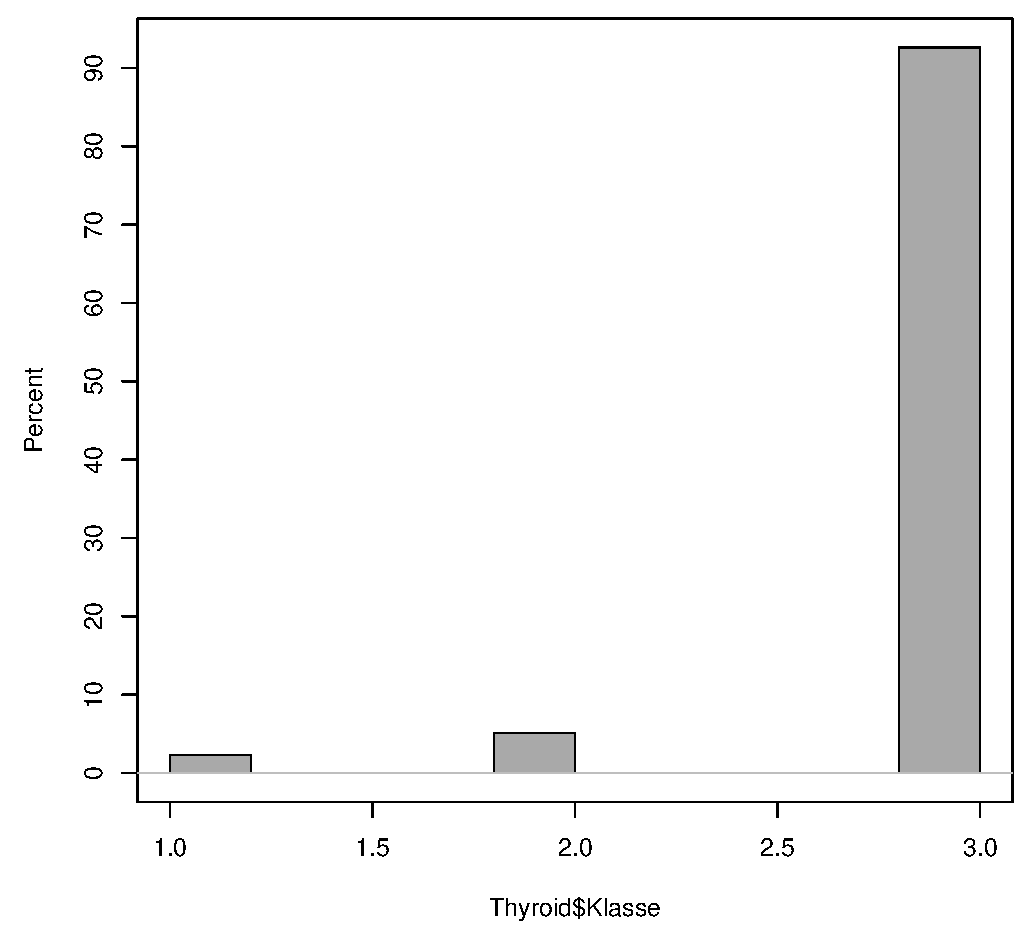
\includegraphics[width=0.6\textwidth]{../images/klassen-verteilung}
  \caption{Häufigkeitsverteilung der Klassen}
  \label{fig:klassen-verteilung}
\end{figure}

\section{Entwurf eines neuronalen Netzes}
Für die folgenden Versuche wird ein künstliches neuronales Netz vom Typ
\emph{feed-forward backpropagation} verwendet. Auf die Funktionsweise eines
Feed-Forward-Netzes wird hier nicht näher eingegangen; diese ist u.a. 
beschrieben in \cite{Demuth1998}. Erzeugt wird ein solches Netz mithilfe der 
Neural Network Toolbox in Matlab über den folgenden Funktionsaufruf:

\begin{lstlisting}[numbers=none]
[net, tr, yTrain, eTrain] = newff($PR$, [$S_1$ $S_2$ ... $S_N$], {$TF_1$ $TF_2$ ... $TF_N$}, $BTF$, $BLF$, $PF$)
\end{lstlisting}

Den einzelnen Parametern kommt dabei die folgende Bedeutung zu:

\begin{description}
  \item[$PR$] Eine $R \times 2$ Matrix mit den Minimal- und Maximalwerten der
  $R$ Eingabewerte in der Input-Schicht.
  \item[$S_i$] Größe der $i$-ten Schicht bei insgesamt $N$ Schichten.
  \item[$TF_i$] Aktivierungsfunktion der $i$-ten Schicht, Default: \texttt{tansig}. 
  \item[$BTF$] Trainingsfunktion, Default: \texttt{traingdx}.
  \item[$BLF$] Gewichts-/Schwellwertlernfunktion, Default: \texttt{learngdm}.
  \item[$PF$] Performancefunktion, Default: \texttt{mse}.
\end{description}

Für den Aufbau des Netzes wird zunächst eine \textbf{Eingabeschicht} benötigt, 
in der sich in diesem Falle 21 Neuronen befinden - eines für jedes 
auszuwertende Attribut. Die Anzahl der \textbf{verdeckten Schichten} wird 
zunächst auf 1 festgelegt. In dieser verdeckten Schicht werden 5 Neuronen
eingesetzt. Die Anzahl der Neuronen und der verdeckten Schichten wird in
weiteren Versuchen variiert werden, um eine möglichst optimale Konfiguration zu
finden (s. Listing \ref{tbl:var-neuronen} im Anhang). Für die 
\textbf{Ausgabeschicht} schließlich werden drei binäre Neuronen verwendet. Die 
Werte der einzelnen Neuronen sind dabei entweder 0 oder 1, je nach gewünschter 
Klasse:

\begin{itemize}
  \item Klasse 1: 1-0-0
  \item Klasse 2: 0-1-0
  \item Klasse 3: 0-0-1
\end{itemize} 

\subsection{Trainingsverfahren und -parameter}
Für das initiale Training des Netzes werden die folgenden Trainingsparameter
verwendet\footnote{Nicht aufgeführte Parameter wurden in der Standardeinstellung
belassen}: 

\begin{itemize}
  \item Prozentsatz von Trainingsdaten aus jeder Klasse: 10. Insgesamt 794 
  Datensätze, davon 17 aus Klasse 1, 37 aus Klasse 2 und 667 aus Klasse 3.
  \item Maximale Anzahl Epochen: 2000.
  \item Aktivierungsfunktion $TF_1$: \texttt{logsig}, $TF_2$: \texttt{logsig}.
  \item Trainingsfunktion $BTF$: \texttt{trainrp}.
  \item Performancefunktion $PF$: \texttt{mse}.
  \item Fehlerziel (\texttt{trainParam.goal}): 0.0001.
\end{itemize}

Als Trainingsfunktion wird hier die \textsl{Resilient Backpropagation}-Methode 
eingesetzt, da es nach \cite{Demuth1998} am besten geeignet ist für 
Klassifizierungsaufgaben und auch sehr performant ist. Als Fehlerziel wird MSE =
0.0001 verwendet. Bei MSE handelt es sich um den \emph{Mean Sum Squared Error}
und dieser ist definiert wie folgt: \cite[Kapitel 5]{bittel2007}.

\[
MSE = \frac{1}{N} \sum_{(p,\,t) \in L} (t_i - y_i)^2
\]

In den nachfolgenden Abschnitten sind die Ergebnisse der Testläufe mit der 
initialen Konfiguration sowie Versuche mit variierenden Netzkonfigurationen 
beschrieben.
